\documentclass[a4paper]{report}

\usepackage[french]{babel}
\usepackage[utf8x]{inputenc}
\usepackage[T1]{fontenc}

\usepackage[a4paper,top=3cm,bottom=2cm,left=3cm,right=3cm,marginparwidth=1.75cm]{geometry}

\usepackage{graphicx}


\begin{document}
\pagenumbering{arabic}

\title{Guide utilisateur}
\author{Bastien Chanez}

\maketitle

\renewcommand{\contentsname}{Sommaire}
\tableofcontents


\chapter{Lancement de l'application}
Lancer l'application en cliquant sur l'icône du projet Quizz présent dans les applications de votre appareil.

Le quizz se lance et on arrive sur la page d'accueil de l'application quizz. 
La page d'accueil de l'application quizz affiche trois boutons, le bouton "Jouer", le bouton "Gerer" et le bouton "Quitter".

\begin{figure}[h]
\centering
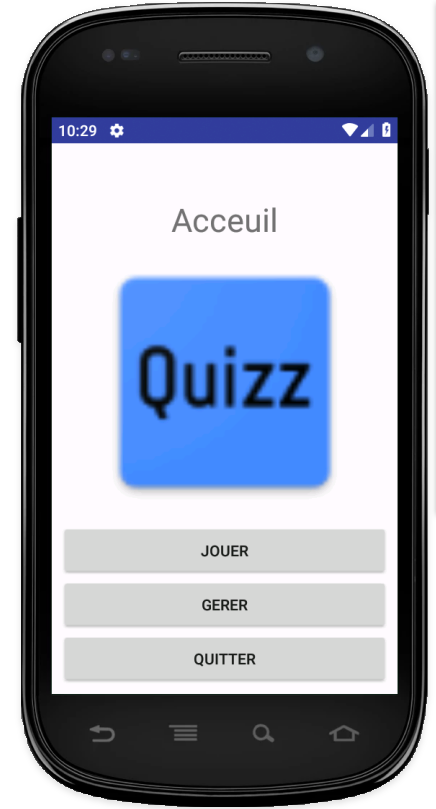
\includegraphics[width=0.3\textwidth]{accueil.png}
\caption{\label{fig:Accueil}Page d'accueil de l'application Quizz.}
\end{figure}

\textbf{Le bouton "Jouer"}, pour jouer un quizz en répondant à des questions.\\
\textbf{Le bouton "Gerer"}, pour gérer les quizzs en les éditant.\\
\textbf{Le bouton "Quitter"}, pour quitter l'application.	

\chapter{Jouer un quizz}
Pour jouer un quizz, cliquer sur le bouton "Jouer" présent sur la page d'accueil.

Vous arrivez sur la page de sélection du quizz pour choisir le quizz que vous voulez jouer.

\section{Sélectionner un quizz}
La page de sélection du quizz vous affiche une liste de quizz ainsi qu'un bouton retour.

\begin{figure}[h]
\centering
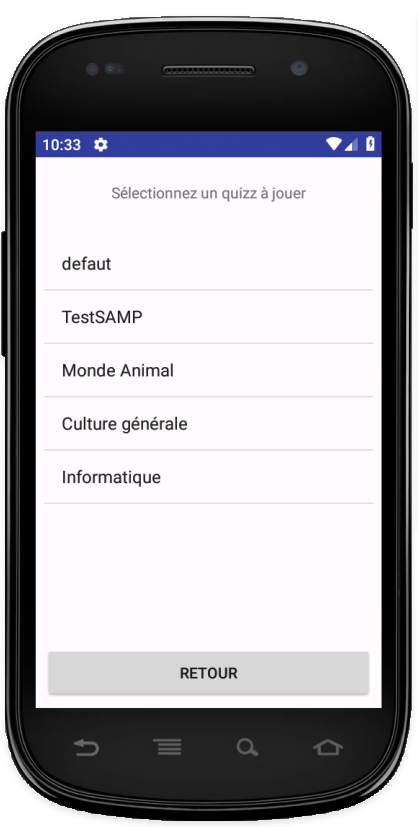
\includegraphics[width=0.3\textwidth]{jouerSelectQuizz.png}
\caption{\label{fig:Sélection du quizz pour jouer}Page de sélection du quizz pour jouer.}
\end{figure}

\textbf{La liste de quizz}, une fois un quizz sélectionné, jouera le quizz.\\
\textbf{Le bouton "retour"}, retourne à la page d'accueil de l'application Quizz présenté lors du lancement de l'application.\\

Remarque : Au lancement de l'application si vous n'avez pas téléchargé les quizzs, il ne vous est proposé que le quizz "défaut".


\newpage
\section{Jouer}
La page pour jouer vous affiche le score, une question, une liste de réponses et un bouton retour.

\begin{figure}[h]
\centering
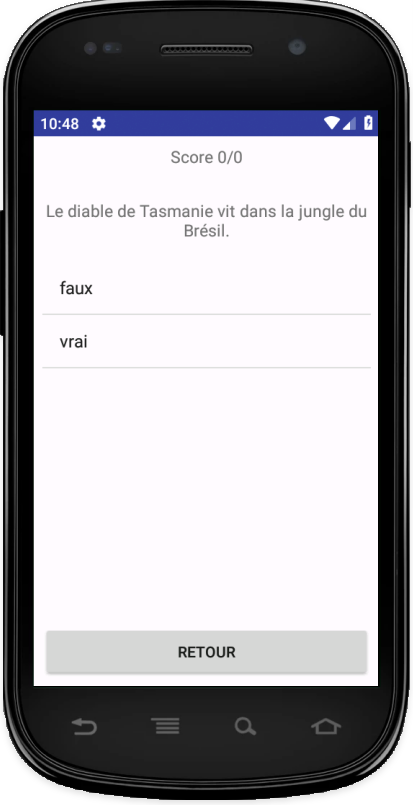
\includegraphics[width=0.3\textwidth]{jouer.png}
\caption{\label{fig:Jouer}Page pour jouer le quizz.}
\end{figure}

\textbf{Le score}, affiche le score de la partie actuelle, ce score est calculé de la façon suivante : \\
nombre de questions répondues justes / nombre de questions répondues \\
\textbf{Une question}, affiche les questions du quizz sélectionné précédemment chacun leur tour jusqu'à que vous ayez répondu à toutes les questions. \\
\textbf{Une liste des réponses}, affiche les réponses proposé pour la question en cours, sélectionner une réponse pour répondre à la question. \\
\textbf{Un bouton retour}, quitte le jeu et retourne à la page de sélection du quizz.\\


\newpage
\section{Réponse juste}
Lorsque votre réponse est bonne, un toast apparaît pour vous l'informer et le score augmente.

\begin{figure}[h]
\centering
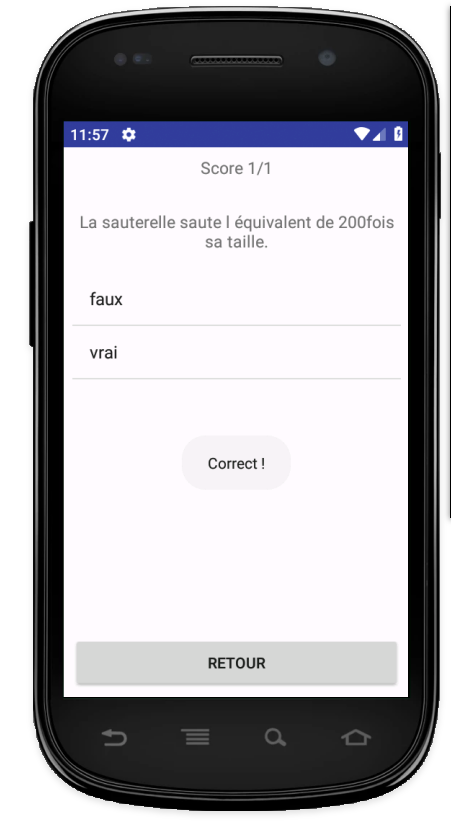
\includegraphics[width=0.3\textwidth]{reponseJuste.png}
\caption{\label{fig:Réponse juste}Réponse juste.}
\end{figure}


\newpage
\section{Réponse fausse}
Lorsque votre réponse est fausse, un toast apparaît pour vous l'informer et le score n'augmente pas.

\begin{figure}[h]
\centering
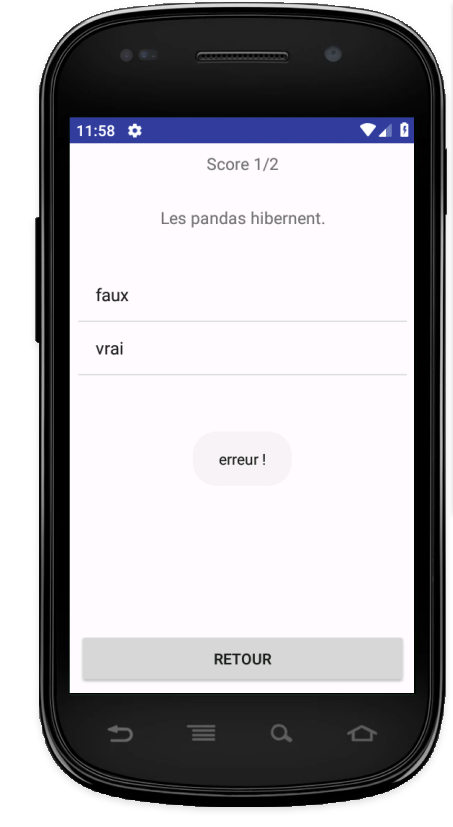
\includegraphics[width=0.3\textwidth]{reponseFausse.png}
\caption{\label{fig:Réponse fausse}Réponse fausse.}
\end{figure}


\newpage
\section{Page de fin du quizz}
Une fois toutes les questions du quizz choisie répondu, une page s'affiche avec le score total, le message "fin" et un bouton retour.

\begin{figure}[h]
\centering
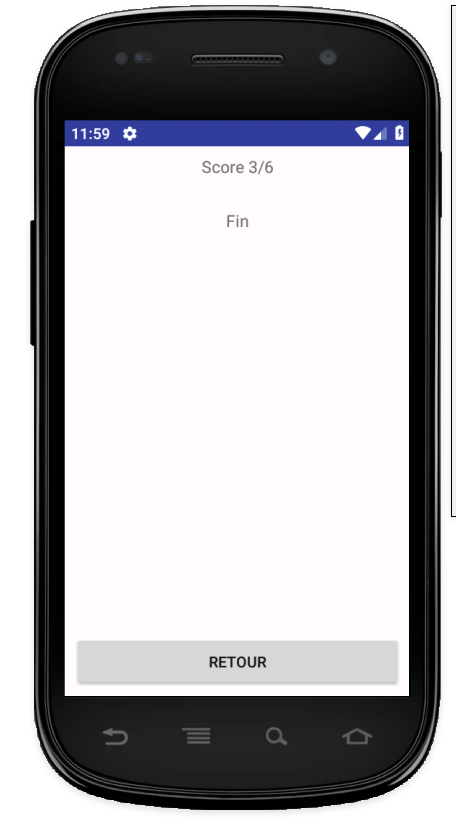
\includegraphics[width=0.3\textwidth]{finJeu.png}
\caption{\label{fig:Page de fin du quizz}Page de fin du quizz.}
\end{figure}

\textbf{Le score}, affiche le score total de la partie, ce score est calculé de la façon suivante : \\
nombre de questions répondues justes / nombre de questions répondues \\
\textbf{le message "fin"}, annonce la fin de la partie. \\
\textbf{Un bouton retour}, retourne à la page de sélection du quizz.\\

\chapter{Gérer les quizzs}
Pour gérer les quizzs, cliquer sur le bouton "Gerer" présent sur la page d'accueil.

Vous arrivez sur la page de sélection du quizz pour choisir le quizz que vous voulez éditer.

\section{Sélectionner un quizz}
La page de sélection du quizz vous affiche une liste de quizz, le bouton "nouveau", le bouton "télécharger" ainsi qu'un bouton retour.

\begin{figure}[h]
\centering
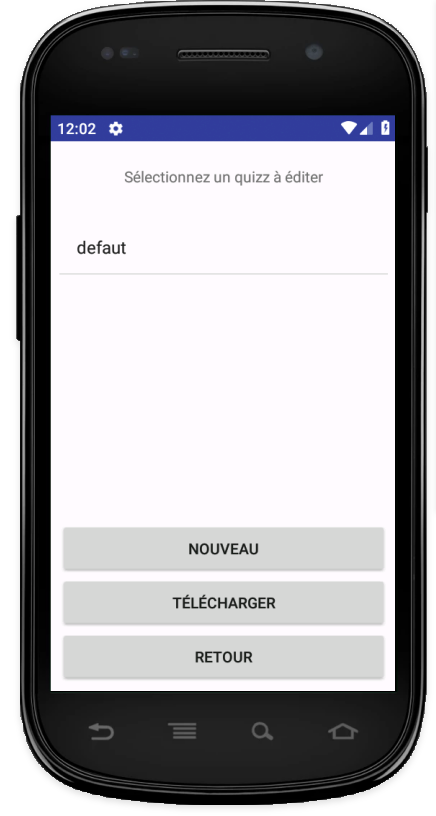
\includegraphics[width=0.3\textwidth]{gererSelectQuizz.png}
\caption{\label{fig:Sélection du quizz pour l'éditer}Page de sélection du quizz pour l'éditer.}
\end{figure}

\textbf{La liste de quizz}, sélectionner un quizz, pour l'éditer.\\
\textbf{Le bouton "nouveau"}, crée un nouveau quizz. \\
\textbf{Le bouton "télécharger"}, télécharge des quizzs supplémentaires. \\
\textbf{Le bouton "retour"}, retourne à la page d'accueil de l'application Quizz présenté lors du lancement de l'application. \\

Remarque : Au lancement de l'application si vous n'avez pas téléchargé les quizzs, il ne vous est proposé que le quizz "défaut".


\newpage
\section{Nouveau quizz}
La page de nouveau quizz affiche un champ texte, le bouton "créer" et le bouton "retour".

\begin{figure}[h]
\centering
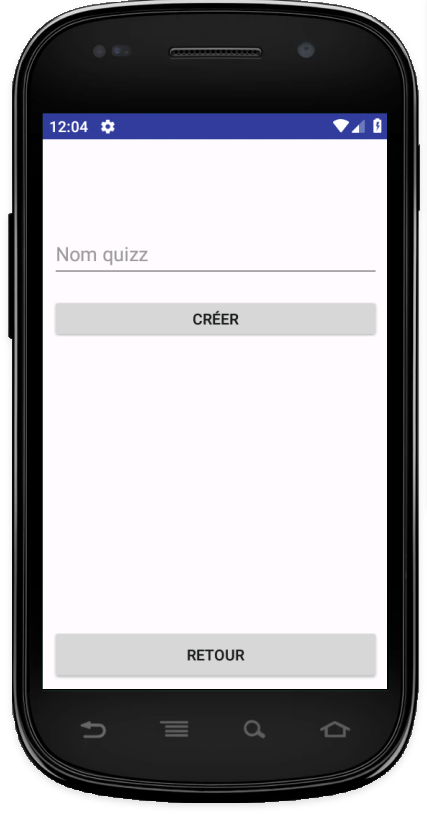
\includegraphics[width=0.3\textwidth]{newQuizz.png}
\caption{\label{fig:Nouveau quizz}Page de création d'un nouveau quizz.}
\end{figure}

\textbf{Le champ texte}, rentrer le nom du quizz dans ce champ. \\
\textbf{Le bouton "créer"}, créer le nouveau quizz avec le nom renseigné dans le champ texte et retourne à la page de sélection du quizz pour l'éditer. \\
\textbf{Le bouton retour}, retourne à la page de sélection du quizz pour l'éditer. \\


\newpage
\section{Éditer un quizz}
La page d'édition d'un quizz affiche un champ texte, le bouton "modifier", le bouton "supprimer", une liste de questions, le bouton "nouveau" et le bouton "retour".

\begin{figure}[h]
\centering
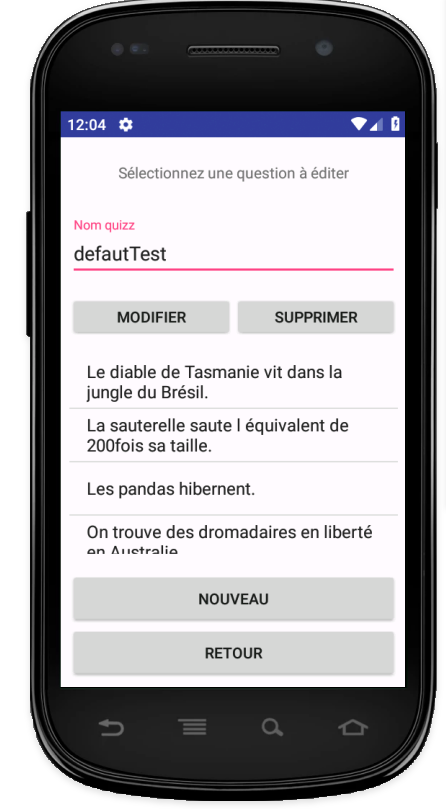
\includegraphics[width=0.3\textwidth]{editerQuizz.png}
\caption{\label{fig:Éditer un quizz}Page d'édition d'un quizz.}
\end{figure}

\textbf{Le champ texte}, modifier le nom du quizz sélectionné précédemment. \\
\textbf{Le bouton "modifier"}, modifie le quizz et retourne à la page de sélection du quizz pour l'éditer. \\
\textbf{Le bouton "supprimer"}, supprime le quizz et retourne à la page de sélection du quizz pour l'éditer. \\
\textbf{La liste de questions}, affiche les questions concernées par ce quizz, cliquer dessus pour éditer une question. \\
\textbf{Le bouton "nouveau"}, créer une nouvelle question pour ce quizz. \\
\textbf{Le bouton "retour"}, retourne à la page de sélection du quizz pour l'éditer. \\


\newpage
\section{Nouvelle question}
La page de nouvelle question affiche un champ texte, le bouton "créer" et le bouton "retour".

\begin{figure}[h]
\centering
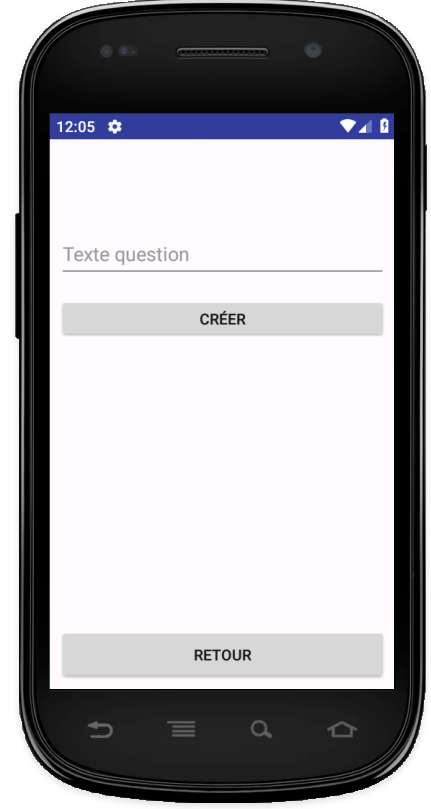
\includegraphics[width=0.3\textwidth]{newQuestion.png}
\caption{\label{fig:Nouvelle question}Page de création d'une nouvelle question.}
\end{figure}

\textbf{Le champ texte}, rentrer le nom de la question dans ce champ. \\
\textbf{Le bouton "créer"}, créer la nouvelle question avec le nom renseigné dans le champ texte et retourne à la page d'édition du quizz concerné. \\
\textbf{Le bouton retour}, retourne à la page d'édition du quizz concerné. \\


\newpage
\section{Éditer une question}
La page d'édition d'une question affiche un champ texte, le bouton "modifier", le bouton "supprimer", une liste de réponses, le bouton "nouveau" et le bouton "retour".

\begin{figure}[h]
\centering
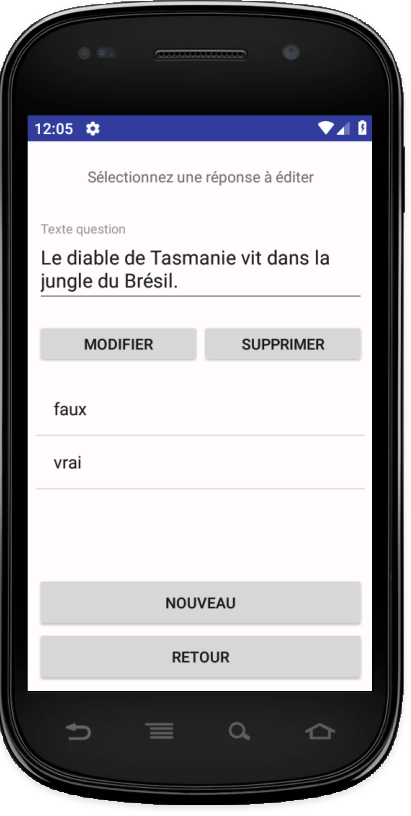
\includegraphics[width=0.3\textwidth]{editerQuestion.png}
\caption{\label{fig:Éditer une question}Page d'édition d'une question.}
\end{figure}

\textbf{Le champ texte}, modifier le nom de la question sélectionnée précédemment. \\
\textbf{Le bouton "modifier"}, modifie la question et retourne à la page d'édition du quizz concerné. \\
\textbf{Le bouton "supprimer"}, supprime la question et retourne à la page de sélection du quizz concerné. \\
\textbf{La liste de réponses}, affiche les réponses concernées par cette question, cliquer dessus pour éditer une réponse. \\
\textbf{Le bouton "nouveau"}, créer une nouvelle réponse pour cette question. \\
\textbf{Le bouton "retour"}, retourne à la page d'édition du quizz concerné. \\


\newpage
\section{Nouvelle réponse}
La page de nouvelle réponse affiche un champ texte, un switch, le bouton "créer" et le bouton "retour".

\begin{figure}[h]
\centering
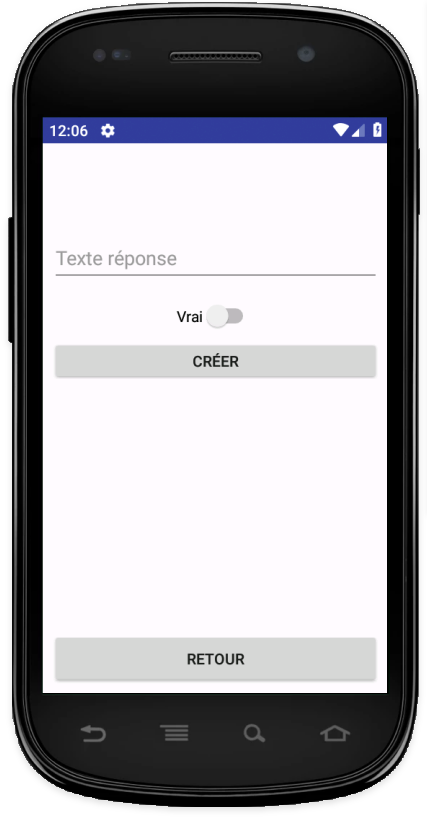
\includegraphics[width=0.3\textwidth]{newReponse.png}
\caption{\label{fig:Nouvelle réponse}Page de création d'une nouvelle réponse.}
\end{figure}

\textbf{Le champ texte}, rentrer le nom de la réponse dans ce champ. \\
\textbf{Le switch}, cocher pour que la réponse soit une bonne réponse et décocher pour que la réponse soit une mauvaise réponse. \\
\textbf{Le bouton "créer"}, créer la nouvelle réponse avec le nom renseigné dans le champ texte et retourne à la page d'édition de la question concernée. \\
\textbf{Le bouton retour}, retourne à la page d'édition de la question concernée. \\


\newpage
\section{Éditer une réponse}
La page d'édition d'une réponse affiche un champ texte, un switch, le bouton "modifier", le bouton "supprimer" et le bouton "retour".



\begin{figure}[h]
\centering
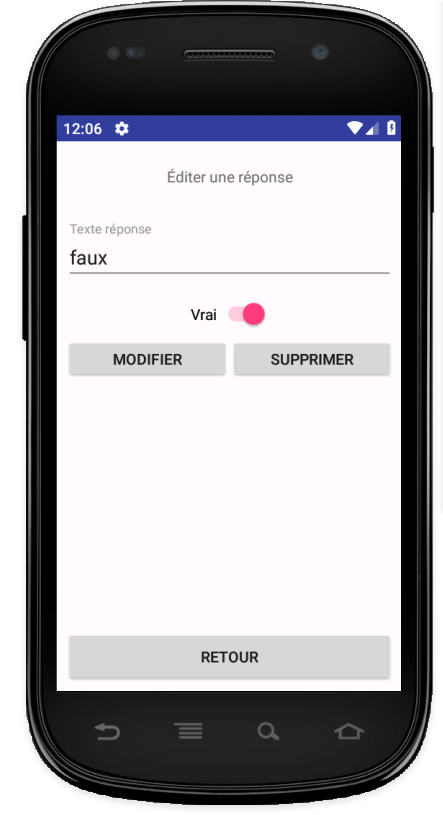
\includegraphics[width=0.3\textwidth]{editerReponse.png}
\caption{\label{fig:Éditer une réponse}Page d'édition d'une réponse.}
\end{figure}

\textbf{Le champ texte}, modifier le nom de la réponse sélectionnée précédemment. \\
\textbf{Le switch}, cocher pour que la réponse soit une bonne réponse et décocher pour que la réponse soit une mauvaise réponse. \\
\textbf{Le bouton "modifier"}, modifie la réponse et retourne à la page d'édition de la question concernée. \\
\textbf{Le bouton "supprimer"}, supprime la réponse et retourne à la page d'édition de la question concernée. \\
\textbf{Le bouton "retour"}, retourne à la page d'édition de la question concernée. \\

\chapter{Quitter l'application}
Pour quitter l'application, cliquer sur le bouton "Quitter" présent sur la page d'accueil.

\renewcommand{\listfigurename}{Tables des illustrations}
\listoffigures

\end{document}
